\documentclass[a4paper,11pt]{article}
\usepackage{graphicx}
\usepackage{booktabs}
\usepackage{setspace}
\usepackage{parskip}
\onehalfspacing
\begin{document}

\author{Hiromasa Okada}
\title{\vspace{-2cm}Report for Sheet 1\\
\small{Lab Course Machine Learning and Data Analysis}}
\maketitle
\section*{Implementation comments}

I have implemented PCA, AUC LLE and Gamma-index. AUC LLE and Gamma-index are simply implemented by functions but PCA is by class. If we create a PCA class with $pca = PCA(X)$ where $X$ is dataset with nxd (n is number of data points and d is the dimension of a data point), the programm saves  principle components and eigenvalue in objects. This class has two other functions $projection(self, X, m)$ and $denoise(self, X, m)$ where $m$ is number of dimension to which we will reduce. Projection is used for dimension reduction by using the saved principal components and denoise is used for denoising by reconstruction from the projected data points. \\
The function $auc(y_true, y_val, plot=False)$ where $ytrue$ is label array and $yval$ is value array returns AUC. If $plot$ is true it shows also ROC graph. \\
The function $lle(X, m, tol, n_rule='knn', k=5, epsilon=1.)$ returns in m dimension embedded data points. If a rule $knn$ is choosen, during the lle k-neighbors are choosen or if a rule $eps_ball$ is choosen, the neighbors in a distance "epsilon" are choosen.

By the test programm the principal components of PCA are not same as the $Ucorrect$ but my programm has the same result as the result of scikit-learn's principal components.

\begin{verbatim}
import sheet1 as imp
print("Principle conponents of my inplementaion")
pca = imp.PCA(X)
print(pca.U)
print("correct Principle conponents")
print(correct_U)
p= sklearn.decomposition.PCA()
p.fit(X)
aaa = -p.components_
print("Principle conponents by scikit-learn")
print(-p.components_)

Principle conponents of my inplementaion
[[-0.3655603   0.85514315 -0.36755389]
 [ 0.79651591  0.49171606  0.35182059]
 [-0.48158911  0.16415088  0.86088699]]
correct Principle conponents
[[ 0.3655603  -0.85514315  0.36755389]
 [-0.79651591 -0.49171606 -0.35182059]
 [-0.48158911  0.16415088  0.86088699]]
Principle conponents by scikit-learn
[[-0.3655603   0.85514315 -0.36755389]
 [ 0.79651591  0.49171606  0.35182059]
 [-0.48158911  0.16415088  0.86088699]]
\end{verbatim}


\section*{Assignment 5}
In this assignment, I analyzed the usps dataset with PCA.
\subsection*{1. Load the usps data set.}
With following code I loaded data set X (nxd) where d is dimension and n is number of data points.
\begin{verbatim}
from scipy.io import loadmat
#1. Load the usps data set.
data = loadmat('usps.mat') 
label = data['data_labels']
pat = data['data_patterns']
\end{verbatim}
\subsection*{2. Analysis of PCA}

But to be accepted, X must be transposed before calicurating PCA.
\begin{verbatim}
#2. Analysis of PCA:
pca = imp.PCA(pat.T)
\end{verbatim}
Now princile components are calicurated.
Next visualize all principal values, the largest 25 principal values and the first 5 principal directions.

\begin{verbatim}
#(a) Visualize all principal values,
plt.figure(0, (16,4))
cut = len(pca.D)
plt.bar(np.arange(cut), pca.D[:cut], lw=0)
plt.title("eigenvalues")
plt.show()

#(b) Visualize the largest 25 principal values 
plt.figure(0, (16,4))
cut = min(len(pca.D),25)
plt.bar(np.arange(cut), pca.D[:cut], lw=0)
plt.title("eigenvalues")
plt.show()
\end{verbatim}

\begin{figure}[htbp]
  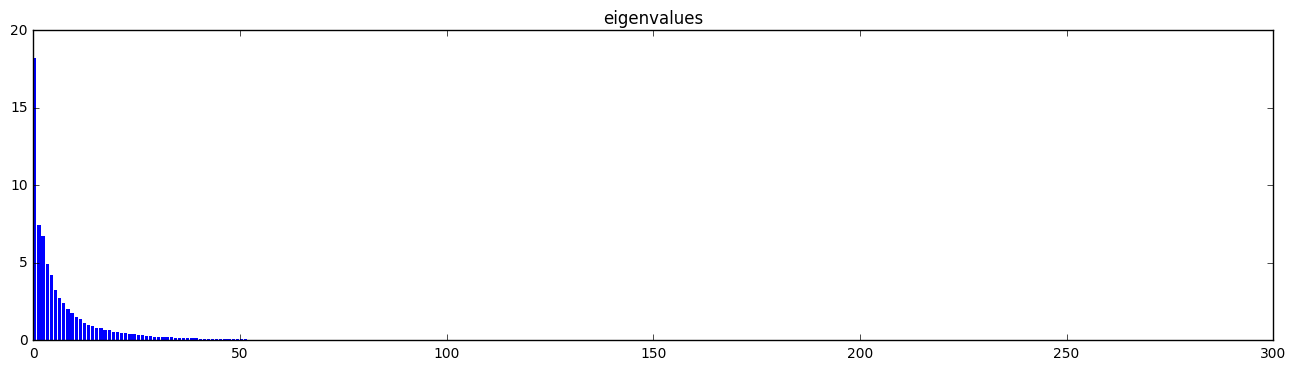
\includegraphics[scale=0.4]{allpc.png}
  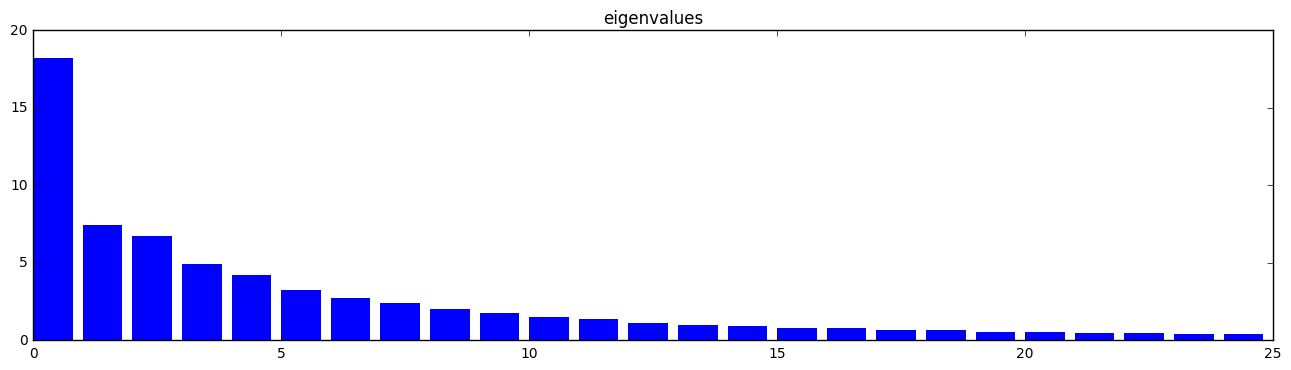
\includegraphics[scale=0.4]{5pc.png}
\end{figure}

\begin{verbatim}

\end{verbatim}

From these graphs we know the first largst principal value is much larger than second largest value and following. It means that the principal direction with the largest principal value is the most correlated direction. Principle value means also variance so that it shows this direction is the largest.  \\ 

\begin{verbatim}
#(c) the first 5 principal directions (as images, see imshow).
plt.figure(figsize=(48,32))
for i in range(5):
    plt.subplot(16,16,i+1)
    plt.title("eigenvector %i" % (i+1))
    plt.imshow(pca.U.T[:,i].reshape(16,16))
\end{verbatim}


\begin{figure}[htbp]
  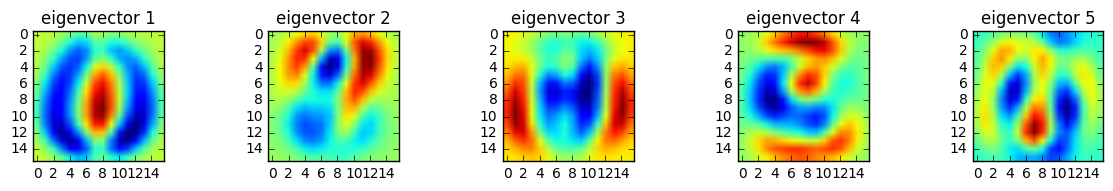
\includegraphics[scale=0.4]{5eigv.png}
  \caption{First 5 Principle directions}
\end{figure}

\subsection*{3. Consider three noise scenarios}
First I made noised images and an example is following.
\begin{figure}[htbp]
  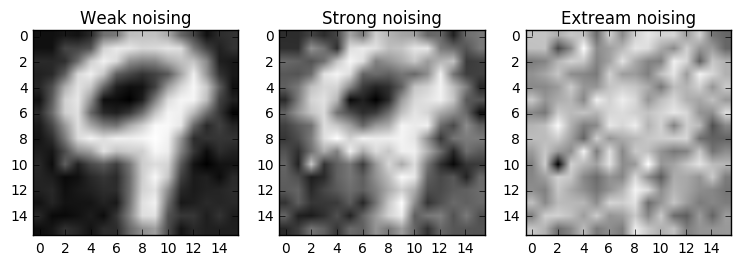
\includegraphics[scale=0.4]{noisimg.png}
  \caption{Example of a noised image}
\end{figure}

After PCA computation I got following values of principal palues. \\
From this results we know that small principal values are differ from each others but large values are almost same. Therefore large value corresponding principal direction has features of original data and small value corresponding principal values shuld be noises.
\begin{figure}[htbp]
  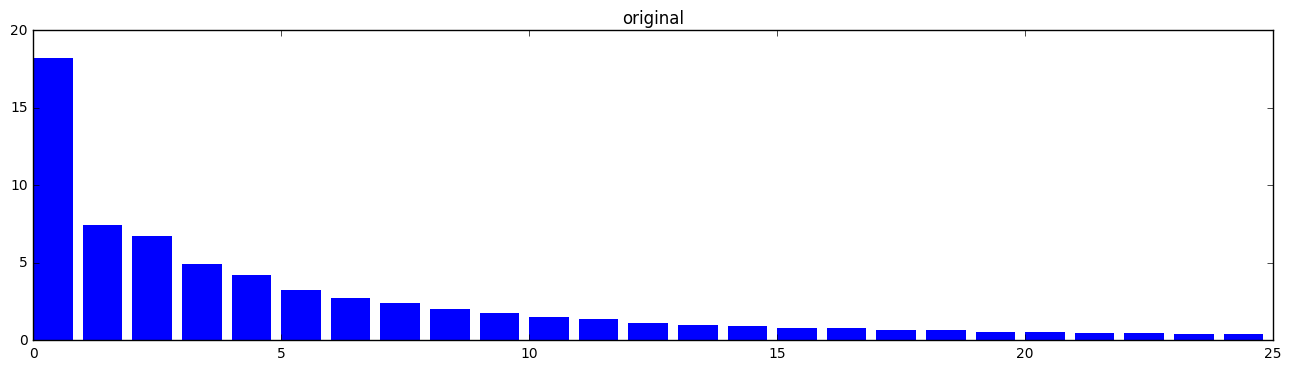
\includegraphics[scale=0.4]{orgev.png}
  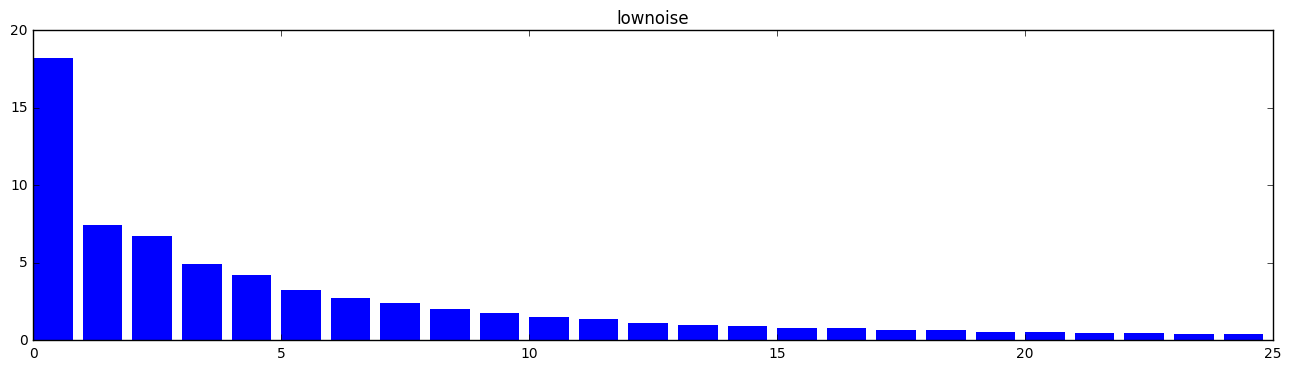
\includegraphics[scale=0.4]{lowev.png}
  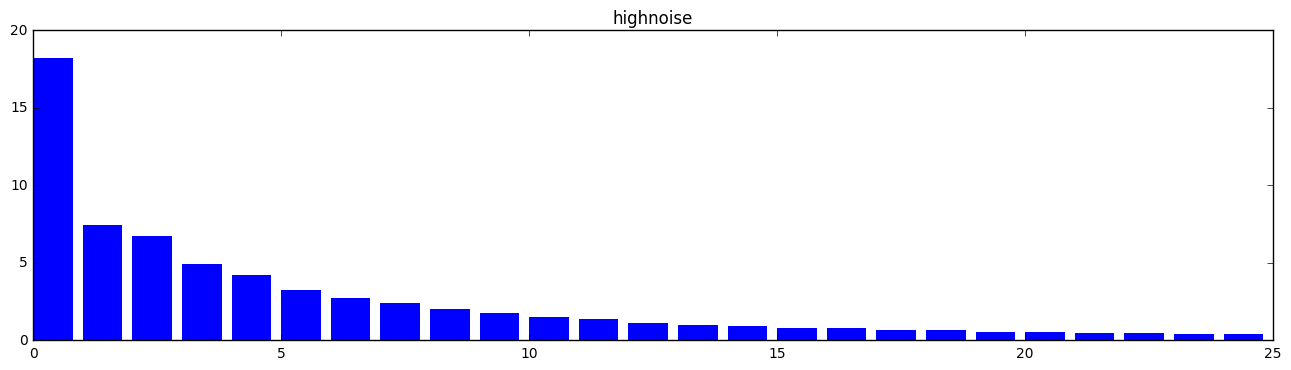
\includegraphics[scale=0.4]{stev.png}
  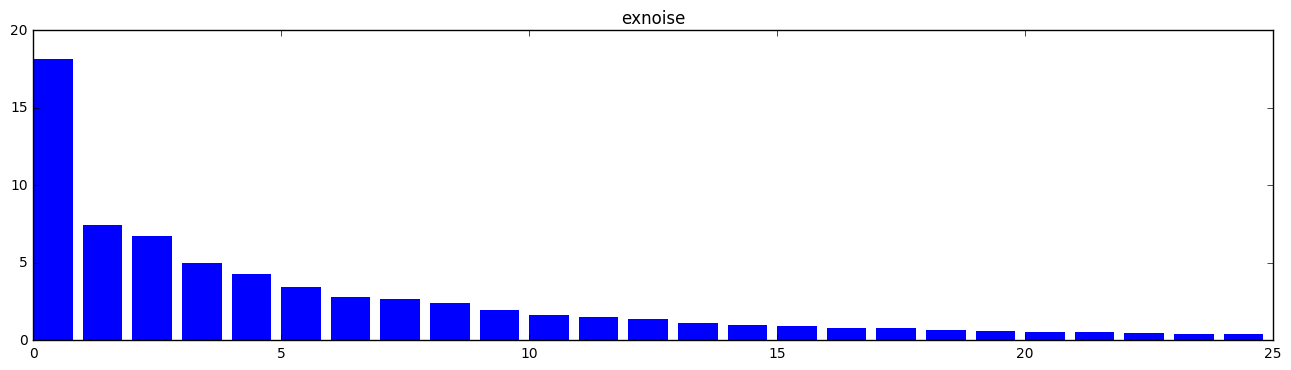
\includegraphics[scale=0.4]{exev.png}
  \caption{Example of largest 5 principle values}
\end{figure}

\begin{figure}[htbp]
  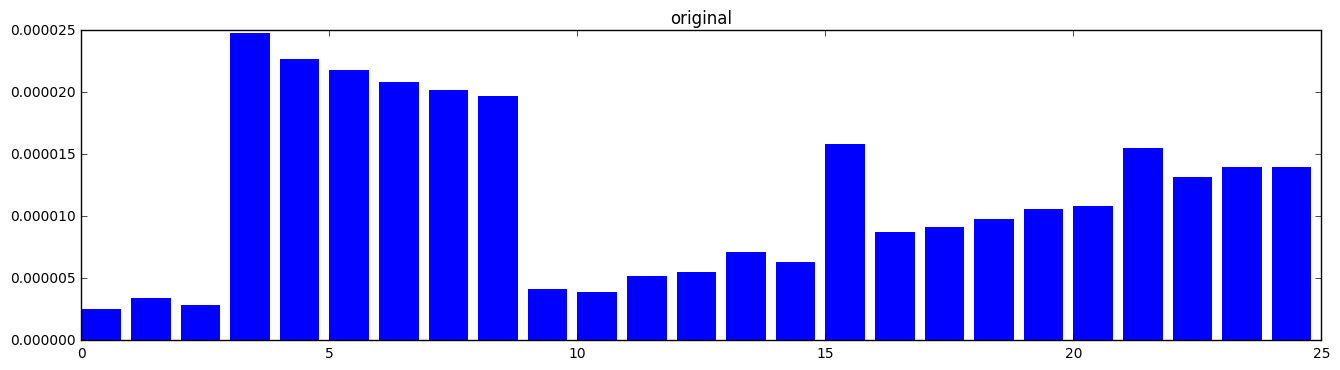
\includegraphics[scale=0.4]{orgev2.png}
  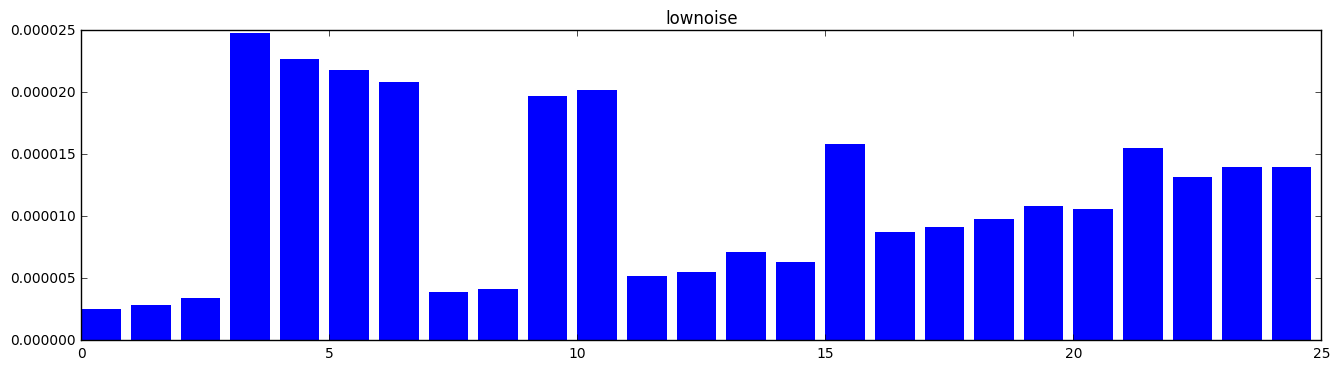
\includegraphics[scale=0.4]{lowev2.png}
  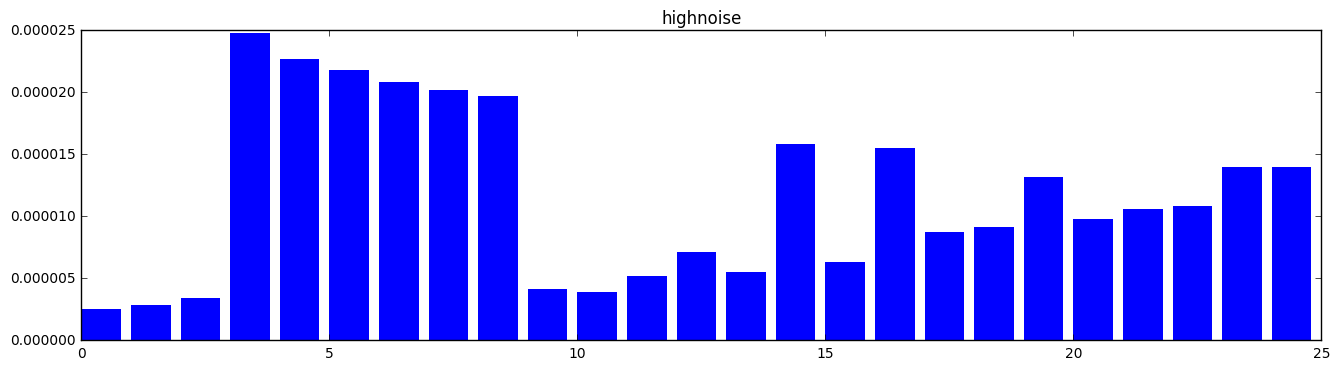
\includegraphics[scale=0.4]{stev2.png}
  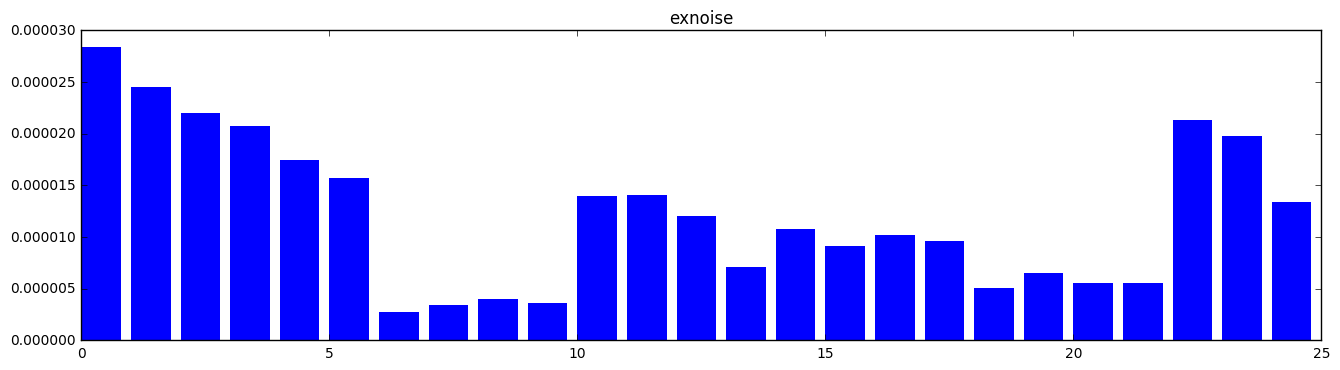
\includegraphics[scale=0.4]{exev2.png}
   \caption{Example of smallest 5 principle values}
\end{figure}
\subsection*{4. Define m}
Now I'd like to find the number $m$ how many principal components are used for denoising. For each noise case, to find m I tried from m=1 to m=100 and calicurated average errors between reconstructed points and original data points. \\
In every case the errors are smaller, when m is more. But from around m=25 


\begin{figure}[htbp]
  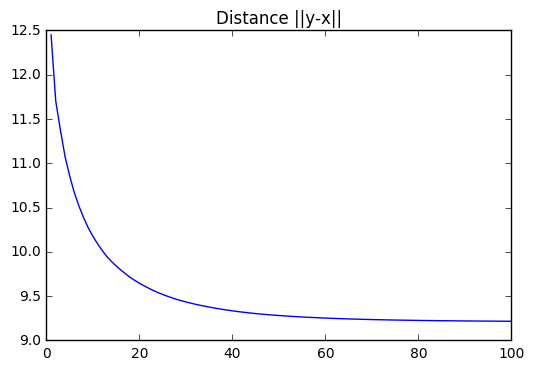
\includegraphics[scale=0.7]{dlown.png}
  \caption{Distance between original and from lownoise reconstructed}
  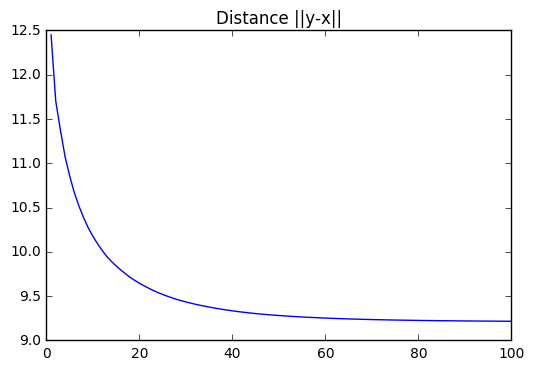
\includegraphics[scale=0.7]{dh.png}
  \caption{Distance between original and from strong noise reconstructed}
  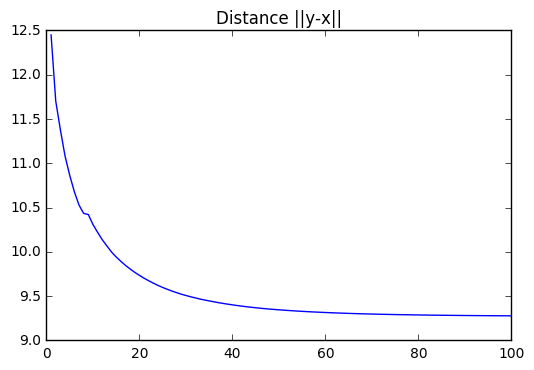
\includegraphics[scale=0.7]{de.png}
  \caption{Distance between original and from extream noise reconstructed}
\end{figure}


\end{document}
